\section{Actividad 6}


\subsection*{a) Calcular la densidad espectral de potencia y la función autocorrelación de $n(t)$. Graficar que se obtiene a la salida de cada filtro y del modulador producto (no debe usar el programa).} 

	\begin{figure}[h!]
		\centering
		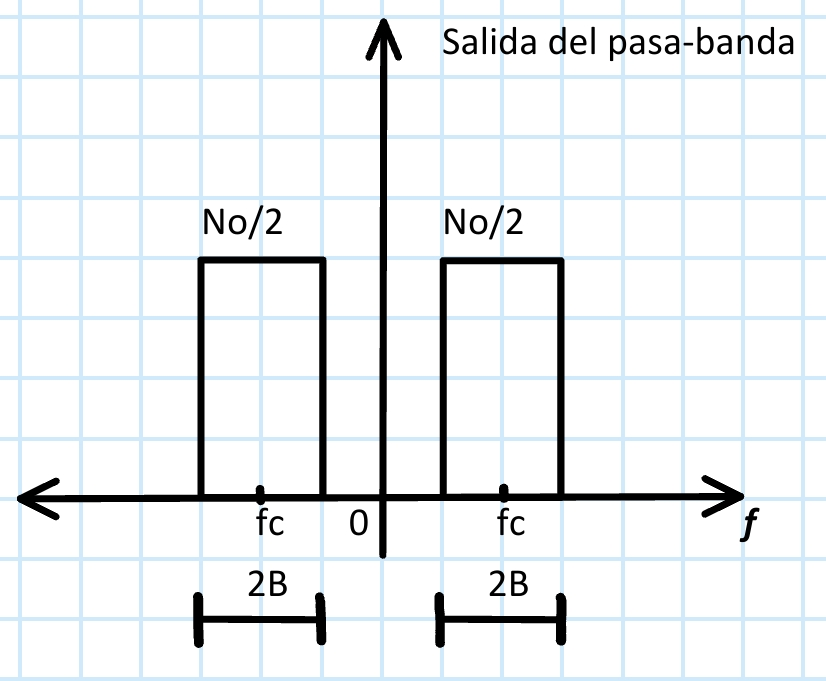
\includegraphics[width=7cm]{parte_teorica/actividad6_pasabanda.jpg}
		\caption{Densidad espectral de potencia del filtro pasabanda.}
		\label{fig:6pasabanda}
	\end{figure}

    \begin{figure}[h!]
		\centering
		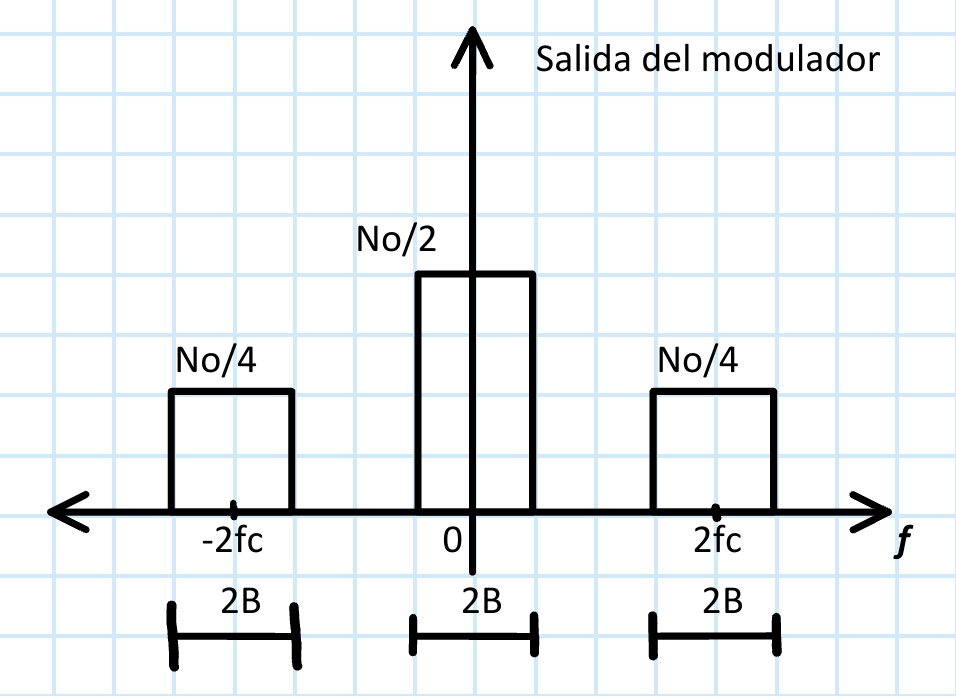
\includegraphics[width=7cm]{parte_teorica/actividad6_modulador.jpg}
		\caption{Densidad espectral salida modulador.}
		\label{fig:6modulador}
	\end{figure}


    \begin{figure}[h!]
		\centering
		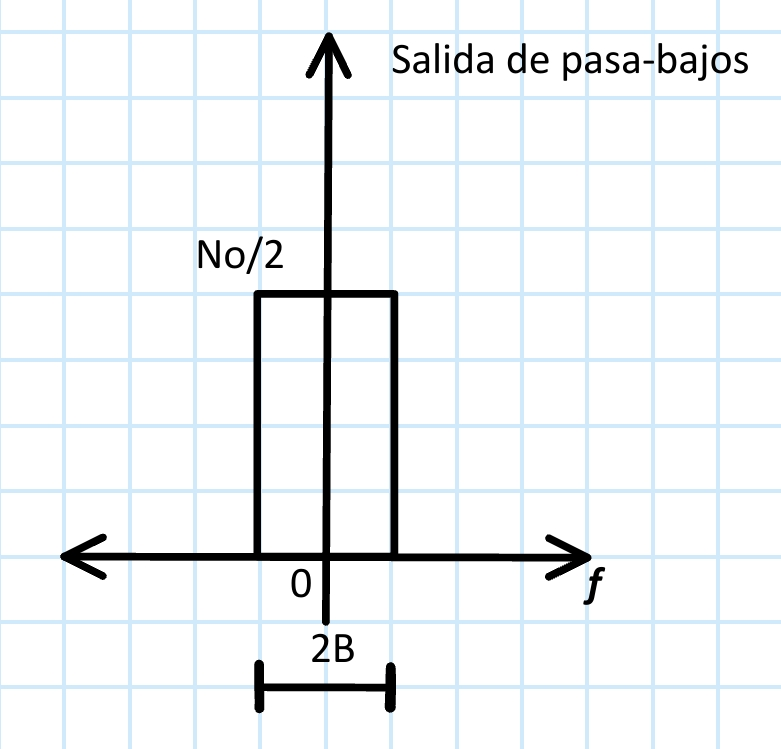
\includegraphics[width=7cm]{parte_teorica/actividad6_pasabajo.jpg}
		\caption{Densidad espectral salida filtro pasa bajo.}
		\label{fig:6pasabajo}
	\end{figure}


\subsection*{b) Calcular la media y la varianza de n(t).}

\subsection*{c) ¿Cuál es la tasa a la cual $n(t)$ puede ser muestreada, de manera tal de que las muestras resultantes sean no correlacionadas?}